\phantomsection
\addcontentsline{toc}{chapter}{Introduction}
\chapter*{Introduction}

This is a thesis in the mathematical sciences, with emphasis on the mathematics.
But before we get to the category theory, I want to say a few, brief words about
the scientific tradition this thesis draws from.

Mathematics is the language of science. New science, new scientific paradigms,
requires new language.

\paragraph{General systems theory.}

General systems theory seeks to talk about composition

While in the past, science tried to explain observable phenomena by reducing them to an interplay of elementary units investigable independently of each other, conceptions appear in contemporary science that are concerned with what is somewhat vaguely termed 'wholeness', i.e. problems of organization, phenomena not resolvable into local events, dynamic interactions manifest in difference of behaviour of parts when isolated or in a higher configuration, etc.; in short, 'systems' of various order not understandable by investigation of their respective parts in isolation. 

von Bertalanffy

It has always had a unification bent to it

Not only are general aspects and viewpoints alike in different sciences; frequently we find formally identical or isomorphic laws in different fields. In many cases, isomorphic laws hold for certain classes or subclasses of 'systems', irrespective of the nature of the entities involved. There appear to exist general system laws which apply to any system of a certain type, irrespective if the particular properties of the system and of the elements involved.

Conventional physics deals only with closed systems, i.e. systems which are considered to be isolated from their environment.

However, we find systems which by their very nature and definition are not closed systems. Every living organism is essentially an open system. It maintains itself in a continuous inflow and outflow, a building up and breaking down of components, never being, so long as it is alive, in a state of chemical and thermodynamic equilibrium but maintained in a so-called steady state which is distinct from the latter.

This dissertation represents the beginnings of an attempt at a category
theoretic framework for general systems theory. A loosely organised body of
research dating back to biologist Ludwig von Bertalanffy in the mid-20th
century \cite{Ber}, general systems theory represents the study of systems built
from rich interconnections of simple component systems. Our central example in
this dissertation will be passive linear circuits: systems built from linear
resistors, inductors, and capacitors.  While each component here is simple,
networks built from such components are complex enough to form the foundation of
modern electronics.

While part of this vision, most notably in von Bertalanffy's home field of
systems biology, has been realised, 


    "Systems biology...is about putting together rather than taking apart, integration rather than reduction. It requires that we develop ways of thinking about integration that are as rigorous as our reductionist programmes, but different....It means changing our philosophy, in the full sense of the term" (Denis Noble).

Feedback; Wiener's cybernetics was often viewed as identical in agenda

More technical progress has been realised: cybernetics, catastrophe theory,
chaos theory, complex systems, network analysis

\paragraph{A diagrammatic approach.}

In this program Odum, diagrams. universal language

what is the algebra of network languages?

hypergraph categories.

graph example

black-boxing, information compression.

examples examples.

Example: trijunction

signal flow

circuits

automata, markov processes, flow networks.

The Yoneda lemma and representability.


Weiner, Cybernetics, Odum, Forrester, SBGN, Rosen, Goguen

\paragraph{A behavioural approach}


Syntactically, by system we mean a `box' with finitely many `ports' through which it
interfaces with the external world. These ports may be of different types. These
systems may be connected together, along ports of the same type, to form larger
systems. Examples of such systems abound; a motivating source of them is
network-style diagrammatic languages, such as the aforementioned electrical
circuit diagrams, but also including chemical reaction networks, Petri nets,
automata, and Markov processes.

We capture this syntactic conception of a system is formally through the notion
of a hypergraph category---a symmetric monoidal category in which every object
is equipped with a special commutative Frobenius monoid in a way compatible with
the monoidal product. This framework provides precise language for describing
how we manipulate and interact with systems.


But what \emph{is} a system, and what do these manipulations and
interconnections mean? Taking inspiration from Willems \cite{Wi} and Deutsch
\cite{D} among others, we consider a system to be merely the set of all possible
different observations one might make by measuring all relevant variables at all
ports of the `box' we use to represent it.  We call this set the
\emph{behaviour} of the system. This arises from a view of physical laws as a
mechanism for simply partitioning the set of all trajectories of a system, the
so-called \emph{universum}, into possible and impossible trajectories.

For example, consider a resistor of resistance $r$. This has two ports---the two
ends of the resistor---and at each port we may measure the potential, and the
current flowing into the port. Now the resistor is governed by Kirchhoff's
current law, or conservation of charge, and Ohm's law. Conservation of charge
states that the current flowing into one port must equal the current flowing out
of the other port, while Ohm's law states that this current will be proportional
to the potential difference, with constant of proportionality $1/r$. Thus the
behaviour of the resistor is the set 
\[
  \big\{\big(\phi_1,\phi_2,
    -\tfrac1r(\phi_2-\phi_1),\tfrac1r(\phi_2-\phi_1)\big)\,\big\vert\,
    \phi_1,\phi_2 \in \mathbb{R}\big\}.
\]
Here the universum is the set
$\mathbb{R}\oplus\mathbb{R}\oplus\mathbb{R}\oplus\mathbb{R}$, where the
summands represent respectively the potentials and currents at each of the two
terminals.

% universum $\mathcal U$ of trajectories, behaviour $\mathcal P(\mathcal U)$,
% principle $\mathcal P(\mathcal P(\mathcal U))$,

The variables associated to each port are determined by the type of the port.
Interconnection of ports then, simply asserts the identification of the
variables at the connected ports. On the level of behaviours, this becomes a
generalised version of composition of relations.

In this thesis I argue that this general framework has wide applicability to
applied science and engineering, and with appropriate additional mathematical
tools allows one to formalise certain diagrammatic languages and their
relationships.



Control theory begins with the following picture:		
\[
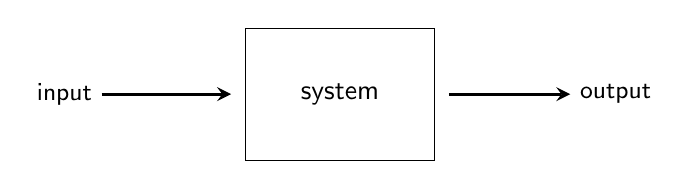
\begin{tikzpicture}
\node(system) [shape=rectangle,draw,inner sep=20pt] at (0,0) {\textsf{system}};
\node(input) at (-3.5,0) {\small{\textsf{input}}};
\node(output) at (3.5,0) {\small{\textsf{output}}};
\draw [->,shorten >=5pt,>=stealth,very thick] (input) 	-- (system);
\draw [->,shorten <=5pt,>=stealth,very thick] (system)	-- (output);
\end{tikzpicture}
\]
In this picture we have an object under study, referred to as a \emph{system}, which when fed certain inputs produces certain outputs. These outputs need not be uniquely determined by the inputs; in general the relationship may be stochastic or non-deterministic, or depend also on internal states of the system. Although we take it as given that the system is an \emph{open} system---so it interacts with its environment, and so we can observe its inputs and outputs---we assume no access to the details of these internal states or the inner workings of the system, and this can add considerable complexity to our models. The end goal of control theory is then to control the system: to understand how to influence its behaviour in order to achieve some desired goal. Two key questions arise: 
\begin{itemize}
\item \textbf{Analysis}: Given a system, what is the relationship it induces between input and output?
\item \textbf{Synthesis}: Given a target relationship between input and output, how do we build a system that produces this relationship?
\end{itemize}
The first, the question of system analysis, provides the basic understanding required to find the inputs that lead to the desired outputs. The second question, the question of synthesis, is the central question of feedback control theory, which aims to design controllers to regulate other systems. We give brief overview of the field, illustrated with some questions of these kinds.

Control has a long history. Indeed, many systems found in the biology and chemistry of living organisms have interesting interpretations from a control theoretic viewpoint, such as those that are responsible for body temperature regulation or bipedal balance \cite{So2}. Human understanding of control developed alongside engineering, and so dates back at least as far as antiquity, with for example the ancient Romans devising elaborate systems to maintain desired water levels in aqueducts \cite{So}. The origin of formal mathematical control theory, however, is more recent, and in general taken to be James Clerk Maxwell's seminal analysis of centrifugal governors, presented to the Royal Society of London in 1868 \cite{CM}. 

A good example of a basic, but characteristic, system studied by control theory,
centrifugal governors were developed to address the problem of speed regulation
for steam engines. A centrifugal governor consists of masses attached via lever
arms to a vertical spindle, as depicted in Figure . This spindle is then connected to the output wheel of an engine, and the height of the masses is inversely related to the aperture of the steam valve into the engine. Higher speeds therefore cause the spindle to rotate faster, which in turn causes the masses to move upward and decrease the flow of steam into the engine. This moderates or prevents acceleration, and hence overspeeding of the engine. Maxwell's paper classifies the possible trajectories over time of the speed of a governed steam engine. 

With respect to the framework laid out above, there are three systems under investigation here. The first is the steam engine, with input steam flow and output engine speed. The second is the centrifugal governor, with input engine speed and output steam flow. The third is the combined governor-steam engine, which forms the main system under investigation, with again input steam flow and output engine speed.

The techniques used and developed from Maxwell's paper, in particular by Rayleigh and Heaviside, are in general known as \emph{transfer function} techniques. A transfer function is a linear map from the set of inputs to the set of outputs of a linear time-invariant system with zero initial conditions. Transfer functions are commonly used in the analysis of single-input single-output linear systems, but become unwieldy or inapplicable for more general systems.

In the 1960s, led by Wiener and Kalman, so-called \emph{state space} techniques were developed to address multiple-input multiple-output, time-varying, nonlinear systems \cite{Fr}. These methods are characterised by defining a system as a collection of input, output, and internal state variables, with the state changing as a function of the input and state variables over time, and the output a function of the input and state. These functions are often implicitly specified by differential equations.

In general, however, classical control theory remains grounded in a paradigm that defines and analyses systems in terms of inputs and outputs or, from another perspective, causes and effects. In recent years Willems, among others, has argued that this input-output perspective is limiting, as in the case of many systems studied through control theory there is no clear distinction between input and output variables \cite{Wi}. For example, given a circuit component for which the relevant variables are the voltages and currents, different contexts may call for the voltage to be viewed as the input and current output, or vice versa. It is useful to have a single framework capable of discussing the behaviour of the component without making this choice.

Moreover, in the drive to understand larger and more complex systems, increasing emphasis has been put on understanding the way systems can be broken down into composite subsystems, and conversely how systems link together to form larger systems \cite{Wi2, KT}. Indeed, interconnection or composition of systems has always played a central role in systems engineering, as in the combination of the centrifugal governor and steam engine of Maxwell's research, and the difficulty of discussing how systems compose within an input-output framework lends support to Willems' call for a more nuanced definition of control system. To illustrate these difficulties, consider the simple example of two water tanks each with two access pipes:
\[
\begin{tikzpicture}
    % draw the tanks
    \begin{pgfonlayer}{main}
    \draw (-4,.1)--(-3,.1)--(-3,0)--(-1,0)--(-1,.1)--(0,.1);
    \draw (-4,.3)--(-3,.3)--(-3,2)--(-1,2)--(-1,.3)--(0,.3);
    \node at (-3,.3) [anchor=-55]{\scriptsize$\begin{array}{c} p_{A1} \\ f_{A1} \end{array}$};
    \node at (-1,.3) [anchor=-125]{\scriptsize$\begin{array}{c} p_{A2} \\ f_{A2} \end{array}$};
    \node at (-2,1){Tank $A$};
    \end{pgfonlayer}
    % fill them with water (in the background)
    \begin{pgfonlayer}{background}
        \filldraw[blue!20] (-4,.1)--(-3,.1)--(-3,0)--(-1,0)--(-1,.1)
        --(0,.1)--(0,.3)--(-1,.3)--(-1,1.8)--(-3,1.8)--(-3,.3)--(-4,.3)
        --cycle;
    \end{pgfonlayer}
\end{tikzpicture}
\qquad
\begin{tikzpicture}
    % draw the tanks
  \begin{pgfonlayer}{main}
    \draw (-4,.1)--(-3,.1)--(-3,0)--(-1,0)--(-1,.1)--(0,.1);
    \draw (-4,.3)--(-3,.3)--(-3,1.7)--(-1,1.7)--(-1,.3)--(0,.3);
    \node at (-3,.3) [anchor=-55]{\scriptsize$\begin{array}{c} p_{B1} \\ f_{B1} \end{array}$};
    \node at (-1,.3) [anchor=-125]{\scriptsize$\begin{array}{c} p_{B2} \\ f_{B2} \end{array}$};
    \node at (-2,1){Tank $B$};
    \end{pgfonlayer}
    % fill them with water (in the background)
    \begin{pgfonlayer}{background}
        \filldraw[blue!20] (-4,.1)--(-3,.1)--(-3,0)--(-1,0)--(-1,.1)
        --(0,.1)--(0,.3)--(-1,.3)--(-1,1.5)--(-3,1.5)--(-3,.3)--(-4,.3)
        --cycle;
    \end{pgfonlayer}
\end{tikzpicture}
\]
For each tank, the relevant variables are the pressure $p$ and the flow $f$. A typical control theoretic analysis might view the water pressure as inducing flow through the tank, and hence take pressure as the input variable, flow as the output variable, and describe each tank as a transfer function $H_\bullet: P_\bullet \to F_\bullet$ between the sets $P_\bullet$ and $F_\bullet$ these vary over. 

Ideally then, the composite system below, connecting pipe 2 of Tank $A$ to pipe 1 of Tank $B$, would be described by the composite of the transfer functions $H_A$ and $H_B$ of these tanks.
\[
\begin{tikzpicture}
    % draw the tanks
    \draw (-4,.1)--(-3,.1)--(-3,0)--(-1,0)--(-1,.1)--(1,.1)--(1,0)--(3,0)--(3,.1)--(4,.1);
    \draw (-4,.3)--(-3,.3)--(-3,2)--(-1,2)--(-1,.3)--(1,.3)--(1,1.7)--(3,1.7)--(3,.3)--(4,.3);
    % fill them with water (in the background)
    \begin{pgfonlayer}{background}
        \filldraw[blue!20] (-4,.1)--(-3,.1)--(-3,0)--(-1,0)--(-1,.1)
        --(1,.1)--(1,0)--(3,0)--(3,.1)--(4,.1)
        --(4,.3)--(3,.3)--(3,1.63)--(1,1.63)--(1,.3)
        --(-1,.3)--(-1,1.7)--(-3,1.7)--(-3,.3)--(-4,.3)
        --cycle;
    \end{pgfonlayer}
    \node at (-3,.3) [anchor=-55]{\scriptsize$\begin{array}{c} p_{A1} \\ f_{A1} \end{array}$};
    \node at (3,.3) [anchor=-125]{\scriptsize$\begin{array}{c} p_{B2} \\ f_{B2} \end{array}$};
    \node at (-1,.3) [anchor=-125]{\scriptsize$\begin{array}{c} p_{A2} \\ f_{A2} \end{array}$};
    \node at (1,.3) [anchor=-55]{\scriptsize$\begin{array}{c} p_{B1} \\ f_{B1} \end{array}$};
    \node at (-2,1){Tank $A$};
    \node at (2,1){Tank $B$};
\end{tikzpicture}
\]
This is rarely the case, and indeed makes little sense: the output of transfer function $H_A$ describes the flow through Tank $A$, while the domain of the transfer function $H_B$ describes pressures through Tank $B$, so taking the output of $H_A$ as the input of $H_B$ runs into data type issues. Instead, here the relationship between the transfer functions $H_A$ and $H_B$, and the transfer function $H_{AB}$ of the composite system can be understood through the fact that connection requires the pressure at pipe 1 of Tank $A$ must be equal to the pressure at pipe 2 of Tank $B$, and that the flow out of the former pipe must equal the flow into the latter---that is, by imposing the relations 
\begin{align*}
p_{A2} &= p_{B1} \\ f_{A2} &= - f_{B1}
\end{align*}
on the variables. Indeed in many contexts, hydraulics and electronics among them, connections between systems are characterised not by the `output' of one system forming the `input' of the next, but by \emph{variable sharing} between the systems. Such relations are often difficult to describe using the language of transfer functions and state space methods.

\section{Outline}

Cospans, decorated cospans, corelations.

\section{Related work}

Category-theoretic frameworks for general systems theory have been developed
before. Notably Goguen and Rosen led efforts. Goguen from a more computer
science perspective, Rosen more in biology.

Most similar is the work of Walters, together with Sabadini and Rosebrugh. In
particular, automata.

\section{Contributions of collaborators}
%Where some part of the thesis is not solely the work of the candidate or has been carried out in collaboration with one or more persons, the candidate shall submit a clear statement of the extent of his or her own contribution.

The first three chapters are my own work. The applications chapters were
developed with collaborators. Chapter 4 arises from a weekly seminar with Paolo
Rapisarda and Pawe\l\ Soboc\'inski. I developed the corelation formalism and provided a
first draft of the paper. Pawe\l\ provided much expertise in signal flow graphs,
significantly revising the text and contributing the section on operational
semantics. Paolo contributed comparisons to classical methods in control theory. 
Much of the text is taken from the paper \cite{FonRapSob16}.

Chapter 5 is joint work with John Baez. John proposed the topic of research, and
supplied some notes on Ohm's law and the principle of minimum power. I
was responsible for producing the first draft of the chapter from this start.
John guided and assisted revisions of this text for publication \cite{BaeFon16}.

I thank my collaborators.
